% Options for packages loaded elsewhere
\PassOptionsToPackage{unicode}{hyperref}
\PassOptionsToPackage{hyphens}{url}
%
\documentclass[
  ignorenonframetext,
]{beamer}
\usepackage{pgfpages}
\setbeamertemplate{caption}[numbered]
\setbeamertemplate{caption label separator}{: }
\setbeamercolor{caption name}{fg=normal text.fg}
\beamertemplatenavigationsymbolsempty
% Prevent slide breaks in the middle of a paragraph
\widowpenalties 1 10000
\raggedbottom
\setbeamertemplate{part page}{
  \centering
  \begin{beamercolorbox}[sep=16pt,center]{part title}
    \usebeamerfont{part title}\insertpart\par
  \end{beamercolorbox}
}
\setbeamertemplate{section page}{
  \centering
  \begin{beamercolorbox}[sep=12pt,center]{part title}
    \usebeamerfont{section title}\insertsection\par
  \end{beamercolorbox}
}
\setbeamertemplate{subsection page}{
  \centering
  \begin{beamercolorbox}[sep=8pt,center]{part title}
    \usebeamerfont{subsection title}\insertsubsection\par
  \end{beamercolorbox}
}
\AtBeginPart{
  \frame{\partpage}
}
\AtBeginSection{
  \ifbibliography
  \else
    \frame{\sectionpage}
  \fi
}
\AtBeginSubsection{
  \frame{\subsectionpage}
}
\usepackage{amsmath,amssymb}
\usepackage{lmodern}
\usepackage{iftex}
\ifPDFTeX
  \usepackage[T1]{fontenc}
  \usepackage[utf8]{inputenc}
  \usepackage{textcomp} % provide euro and other symbols
\else % if luatex or xetex
  \usepackage{unicode-math}
  \defaultfontfeatures{Scale=MatchLowercase}
  \defaultfontfeatures[\rmfamily]{Ligatures=TeX,Scale=1}
\fi
% Use upquote if available, for straight quotes in verbatim environments
\IfFileExists{upquote.sty}{\usepackage{upquote}}{}
\IfFileExists{microtype.sty}{% use microtype if available
  \usepackage[]{microtype}
  \UseMicrotypeSet[protrusion]{basicmath} % disable protrusion for tt fonts
}{}
\makeatletter
\@ifundefined{KOMAClassName}{% if non-KOMA class
  \IfFileExists{parskip.sty}{%
    \usepackage{parskip}
  }{% else
    \setlength{\parindent}{0pt}
    \setlength{\parskip}{6pt plus 2pt minus 1pt}}
}{% if KOMA class
  \KOMAoptions{parskip=half}}
\makeatother
\usepackage{xcolor}
\newif\ifbibliography
\usepackage{longtable,booktabs,array}
\usepackage{calc} % for calculating minipage widths
\usepackage{caption}
% Make caption package work with longtable
\makeatletter
\def\fnum@table{\tablename~\thetable}
\makeatother
\usepackage{graphicx}
\makeatletter
\def\maxwidth{\ifdim\Gin@nat@width>\linewidth\linewidth\else\Gin@nat@width\fi}
\def\maxheight{\ifdim\Gin@nat@height>\textheight\textheight\else\Gin@nat@height\fi}
\makeatother
% Scale images if necessary, so that they will not overflow the page
% margins by default, and it is still possible to overwrite the defaults
% using explicit options in \includegraphics[width, height, ...]{}
\setkeys{Gin}{width=\maxwidth,height=\maxheight,keepaspectratio}
% Set default figure placement to htbp
\makeatletter
\def\fps@figure{htbp}
\makeatother
\setlength{\emergencystretch}{3em} % prevent overfull lines
\providecommand{\tightlist}{%
  \setlength{\itemsep}{0pt}\setlength{\parskip}{0pt}}
\setcounter{secnumdepth}{-\maxdimen} % remove section numbering
\ProvidesPackage{config/presento}
\mode<presentation>

% removing navigation symbols
\setbeamertemplate{navigation symbols}{}

% packages
\usepackage{xcolor}
\usepackage{fontspec}
\usepackage{setspace}
\usepackage{tikz}
\usepackage{multicol}
\usepackage{multirow}

% colors
\definecolor{colorblack}{HTML}{000000} % for note
\definecolor{colorgreen}{HTML}{009933} % for code
\definecolor{colorwhite}{HTML}{FFFFFF} % background
\definecolor{colorblue}{HTML}{0099CC} % blue
\definecolor{colorbig}{HTML}{1f77b4} % for note
\definecolor{colormedium}{HTML}{ff7f0e} % for note
\definecolor{colorsmall}{HTML}{2ca02c} % for note


% font sizes
\newcommand{\fontsizeone}{1em}
\newcommand{\fontsizetwo}{1em}
\newcommand{\fontsizethree}{0.8em}
% line spaces
\newcommand{\linespaceone}{1}

% font families
\newfontfamily{\inconsolatafont}[Path=fonts/]{brill}

% beamer template changes
\setbeamertemplate{frametitle}{
 \vspace{0.40em}
 \noindent
 \hspace{-1.22em}
 \tikz[overlay,remember picture,baseline=0.3em]{\fill[fill= colorblue]  (-0.3,0.05) rectangle (0,0.9); }\color{colorblue}~~\insertframetitle%
}

\setmainfont[Ligatures=TeX,Path=fonts/,
						BoldFont=brillb,
						ItalicFont=brilli,
						BoldItalicFont=brillbi,
						SmallCapsFont=brill]{brill}
\setsansfont[Ligatures=TeX,Path=fonts/,
						BoldFont=brillb,
						ItalicFont=brilli,
						BoldItalicFont=brillbi,
						SmallCapsFont=brill]{brill}
\setmonofont[Color=colorgreen,
						   Scale=0.7,
  						   Path=fonts/]{iosevka-regular}
  
\usepackage[english,russian]{babel}


% frame counter
\newcounter{totalfr}
\setbeamertemplate{footline}{
  \ifnum\inserttotalframenumber=1
    \setcounter{totalfr}{2}
  \else
     \setcounter{totalfr}{\inserttotalframenumber}
  \fi
  \hfill{
    \tikz{
      \filldraw[fill=colorblue!80, draw=colorblue!80]  (0,0) -- (0.2,0) arc (0:{\value{framenumber}*(360/(\value{totalfr}))}:0.2) -- (0,0); 
      \node at (0,0) {\normalsize \color{colorblack}\tiny{\insertframenumber}};
    }
  }
  \hspace{2em}
  \vspace*{1em}
}

% custom commands
\newcommand{\hugetext}[1]{
  {
  \begin{spacing}{\linespaceone}
   \fontsize{\fontsizeone}{\fontsizeone}{ #1}
  \end{spacing}
  }
}

\newcommand{\largetext}[1]{
 {\fontsize{\fontsizetwo}{\fontsizeone}\selectfont{#1}}
}

\newcommand{\setnote}[1]{
 {\fontsize{\fontsizethree}{\fontsizeone}\selectfont\color{colorblack}{#1}}
}

\newcommand{\framecard}[2][colorblue]{
  {\setbeamercolor{background canvas}{bg=#1}
    \begin{frame}[plain]
    \vfill
    \begin{center}
     {#2}
    \end{center}
    \vfill
    \end{frame}
  }
}
\newcommand{\framepic}[3][1]{
  {
    \usebackgroundtemplate{%
    \tikz[overlay,remember picture] \node[opacity=#1, at=(current page.center)] {
      \includegraphics[width=\paperwidth]{#2}};
    }
    \begin{frame}
    #3
    \end{frame}
  }
}
 
  
% Sets the background color to be light gray and the default text color to be heavy dark gray.
% Recommended for presenting with high quality projectors, since the high contrast of black-white is not advisable
\setbeamercolor{background canvas}{bg=colorwhite}
\setbeamercolor{normal text}{fg=colorblack}
\setbeamercolor{title}{fg=colorblue}
\setbeamercolor{subtitle}{fg=colorblue}
\setbeamercolor{author}{fg=colorblack}
\setbeamercolor{alerted text}{fg=colorblue}

\defbeamertemplate*{title page}{customized}[1][]
{
  \vfill
  {\usebeamercolor[fg]{title}\hugetext{\inserttitle}}
  {\usebeamerfont{subtitle}\usebeamercolor[fg]{subtitle}\largetext{\insertsubtitle}\par}
  \vfill
  {\usebeamercolor[fg]{author}\largetext{\insertauthor}}\\
  {\setnote{\insertinstitute}\par}
  \vfill
  {\setnote{\insertdate}\par}
  \vfill
}

\usepackage{natbib}
\bibpunct[: ]{(}{)}{;}{a}{}{,}

\setbeamertemplate{itemize items}{\color{colorblue}$\bullet$}
\setbeamertemplate{enumerate items}{\color{colorblue}$\theenumi$}
\setbeamercolor{block title}{fg=colorblue,bg=white} 
\setbeamertemplate{frametitle continuation}{}

\usepackage{hyperref}
\hypersetup{
    colorlinks=true,
    citecolor=colorblue,
    urlcolor=colorblue
}

\AtBeginSection[]{
\setbeamercolor{background canvas}{bg=colorblue}
\begin{frame}[plain]
  \begin{center}
  \centering
    \usebeamerfont{section title}\huge\insertsection
  \end{center}
\end{frame}
\addtocounter{framenumber}{-1}
\setbeamercolor{background canvas}{bg=colorwhite}
}
\ifLuaTeX
  \usepackage{selnolig}  % disable illegal ligatures
\fi
\usepackage[]{natbib}
\bibliographystyle{apalike}
\IfFileExists{bookmark.sty}{\usepackage{bookmark}}{\usepackage{hyperref}}
\IfFileExists{xurl.sty}{\usepackage{xurl}}{} % add URL line breaks if available
\urlstyle{same} % disable monospaced font for URLs
\hypersetup{
  pdftitle={A corpus of Andi field recordings},
  hidelinks,
  pdfcreator={LaTeX via pandoc}}

\title{A corpus of Andi field recordings}
\author{Samira Verhees¹\\
Aigul Zakirova²\\
George Moroz²\\
Elena Sokur²}
\date{20 September 2022\\
Tbilisi, VI International Conference: Language and Modern Technologies}
\institute{¹Independent researcher, the Netherlands; ²HSE University,
Russia}

\begin{document}
\frame{\titlepage}

\hypertarget{corpora-of-linguistic-convergence-laboratory}{%
\section{\texorpdfstring{\color{colorwhite} Corpora of Linguistic
Convergence
Laboratory}{ Corpora of Linguistic Convergence Laboratory}}\label{corpora-of-linguistic-convergence-laboratory}}

\hypertarget{developing-the-corpus-of-andi}{%
\section{\texorpdfstring{\color{colorwhite} Developing the corpus of
Andi}{ Developing the corpus of Andi}}\label{developing-the-corpus-of-andi}}

\begin{frame}[fragile]{The Andi Language: a sociolinguistic background}
\protect\hypertarget{the-andi-language-a-sociolinguistic-background}{}
\textless{} Avar-Andic \textless{} East Caucasian, glottocode
{[}andi1255{]} spoken in several villages of the Botlikh district of
Dagestan. more than 20,000 speakers of Andi (\citet{aglarov02},
All-Russian National Census 2010) Andi speakers are trilingual in Andi,
Avar and Russian Avar serves as a lingua franca and is taught in school
(Dobrushina et al.~2017)

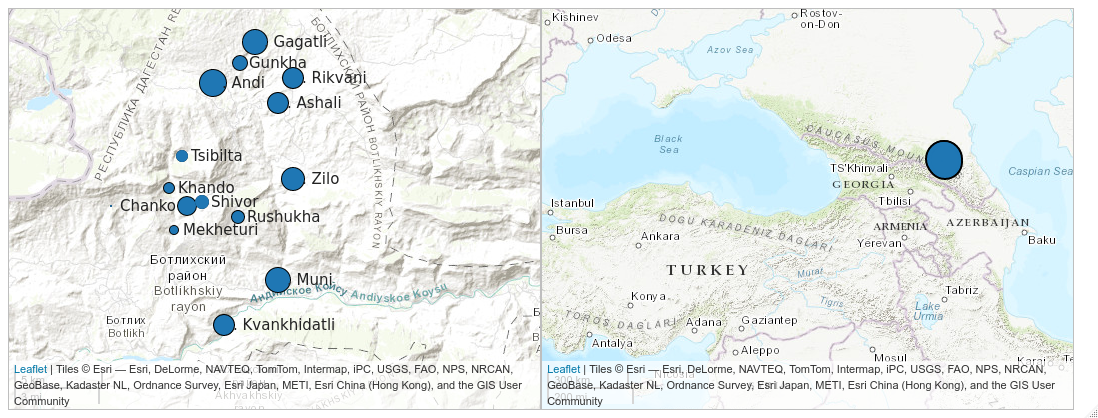
\includegraphics{images/01_map.png}

Created with \texttt{lingtypology} \citep{moroz2017}

\setcounter{footnote}{0}
\end{frame}

\begin{frame}{Andic data}
\protect\hypertarget{andic-data}{}
\begin{longtable}[]{@{}
  >{\raggedright\arraybackslash}p{(\columnwidth - 8\tabcolsep) * \real{0.2340}}
  >{\centering\arraybackslash}p{(\columnwidth - 8\tabcolsep) * \real{0.2872}}
  >{\centering\arraybackslash}p{(\columnwidth - 8\tabcolsep) * \real{0.1809}}
  >{\centering\arraybackslash}p{(\columnwidth - 8\tabcolsep) * \real{0.1489}}
  >{\centering\arraybackslash}p{(\columnwidth - 8\tabcolsep) * \real{0.1489}}@{}}
\toprule()
\begin{minipage}[b]{\linewidth}\raggedright
\end{minipage} & \begin{minipage}[b]{\linewidth}\centering
Andi
\end{minipage} & \begin{minipage}[b]{\linewidth}\centering
Rikvani
\end{minipage} & \begin{minipage}[b]{\linewidth}\centering
Gagatli
\end{minipage} & \begin{minipage}[b]{\linewidth}\centering
Zilo
\end{minipage} \\
\midrule()
\endhead
materials & \citep{kibrik1988, alekseev99} & \citep{suleymanov57} &
\citep{salimov10} & \citep{kayefurth} \\
grammar sketch & + & + & + & + \\
dictionary & + & - & ± & ± \\
morphological parser &
±\footnote[frame]{A pilot version of a morpholoical parser of Andi is presented in (Buntyakova 2022).}
& - & - & - \\
\bottomrule()
\end{longtable}

\setcounter{footnote}{0}
\end{frame}

\begin{frame}{Andic data}
\protect\hypertarget{andic-data-1}{}
\begin{itemize}
\tightlist
\item
  How many hours do we have?
\item
  How many is annotated?
\end{itemize}
\end{frame}

\begin{frame}{Problems}
\protect\hypertarget{problems}{}
\begin{itemize}
\tightlist
\item
  Andi has several dialects and no cross-dialectal standard;

  \begin{itemize}
  \tightlist
  \item
    no full-fledged dictionary
  \item
    no full-fledged grammatical parser (though see a first attempt in
    \citep{buntyakova22})
  \end{itemize}
\item
  Our recorded data are heterogeneous

  \begin{itemize}
  \tightlist
  \item
    different dialects
  \item
    different conventions
  \item
    different file formats
  \end{itemize}
\item
  Due to our limited knowledge of the Andi dialects, sometimes we do not
  know what the correct analysis of a given word form is.
\end{itemize}
\end{frame}

\begin{frame}[fragile]{Solution}
\protect\hypertarget{solution}{}
The material has to be converted to a singular format using
\texttt{phonfieldwork} \citep{moroz20}. For the Andi dialectal corpus
the pipeline is as follows:

\begin{itemize}
\tightlist
\item
  we preprocess the annotation files, converting them to ELAN
  \texttt{.eaf} format \citep{wittenburg06},
\item
  align them with the sound
\item
  gloss them manually or correct mistakes and ambiguities left by
  morphological parser
\item
  publish online using the Tsakorpus platform (Arkhangelskiy 2019)
\item
  repeat all previous steps
\end{itemize}
\end{frame}

\hypertarget{conclusions}{%
\section{\texorpdfstring{\color{colorwhite}
Conclusions}{ Conclusions}}\label{conclusions}}

\begin{frame}{Conclusions:}
\protect\hypertarget{conclusions-1}{}
\end{frame}

\renewcommand\refname{References}
\begin{frame}[allowframebreaks]{References}
  \bibliographytrue
  \bibliography{bibliography.bib}
\end{frame}

\end{document}
